\documentclass[a4paper,twocolumn,10pt]{article}

%% Language and font encodings
\usepackage[english]{babel}
\usepackage[utf8x]{inputenc}
\usepackage[T1]{fontenc}

\usepackage{amsmath,dsfont,bm}

\newcommand{\abbr}[2]{#1 (#2)}
\newcommand{\abbrpl}[2]{#1s (#2)}
\newcommand{\norm}{f}
\newcommand{\normaldist}{\mathcal{N}}
\newcommand{\templateX}{\mathcal X}
\newcommand{\expect}{\mathbb E}
\newcommand{\tx}{\tilde{x}}
\newcommand{\feature}{\mathcal{F}}
\newcommand{\transformer}{\mathcal{T}}
\newcommand{\addgate}{\beta}
\newcommand{\mulgate}{\gamma}
\newcommand{\bx}{\bm{x}}
\newcommand{\std}{\text{std}}
\newcommand{\tX}{\tilde{X}}
\newcommand{\lxl}{\ensuremath{1 \times 1} }

\newcommand{\cX}{\mathcal{X}}
\newcommand{\tcX}{\mathcal{\tilde{X}}}

\newcommand{\zz}{\mathbf{z}}
\newcommand{\yy}{\mathbf{y}}
\newcommand{\xx}{\mathbf{x}}
\newcommand{\txx}{\mathbf{\tilde{x}}}
\newcommand{\R}{\mathds{R}}

\newcommand{\X}{\mathcal{X}}
\newcommand{\Y}{\mathcal{Y}}
\newcommand{\Z}{\mathcal{Z}}
\newcommand{\U}{\mathcal{U}}
\newcommand{\V}{\mathcal{V}}
\newcommand{\F}{\mathcal{F}}
\newcommand{\I}{\mathcal{I}}
\renewcommand{\P}{\mathds{P}}


%% Sets page size and margins
\usepackage[a4paper,top=3cm,bottom=2cm,left=3cm,right=3cm,marginparwidth=1.75cm]{geometry}

%% Useful packages
\usepackage{amsmath}
\usepackage{graphicx}
\usepackage[colorinlistoftodos]{todonotes}
\usepackage[colorlinks=true, allcolors=blue]{hyperref}

\title{Visual Attention: From Classical to Modern Approaches}
\author{Steffen Schneider\\
Technical University of Munich\\
\texttt{steffen.schneider@tum.de}\\
}
\date{}

\begin{document}
\maketitle


\begin{abstract}
  Predicting the ways in which image locations draw the attention of humans gives important insights into the visual system and the way in which humans access image contents.
  The notion of saliency is a popular research item in both neuroscience and lately, also in deep learning research.
  As attention based gating is incorporated in signal processes, predicting saliency to identify important parts of the image is also interesting from a techical perspective.
  In this paper, the implementation of a variant of the Itty Koch model \cite{Itti2000} is discussed as an example for a historical approach to saliency.
  The approach will be compared to a simple data-driven adaptation approach as well as the state-of-the art model for visual saliency, DeepGazeII \cite{Kummerer2017b} according to the MIT300 benchmark.
  The models will be evaluated on a custom dataset of four photographs, three artificial visual stimuli as well as three video files.\footnote{The implementation in Python is available at \texttt{https://github.com/stes/saliency}}\footnote{This report is part of a lab of the Neuroengineering program at TU Munich.}
\end{abstract}

\section{Introduction}

Saliency models usually process an image or a sequency of images and produce a saliency map.

\section{Methods}

In this section, we discuss different methods to compute saliency maps.

To provide a unique mathematical framework, I will consider the architectural similarities of classic approaches such as the Itty Koch model \cite{Itty2000} and modern appraoches such as Deep Gaze \cite{}.

Overall, when given an image $x \in \R^{W\times H \times C}$, many saliency models first use a feature extractor $\F: \R^{W\times H \times C} \mapsto \R^{W\times H \times K}$ to convert an image with $C$ channels into $K$ feature maps.
Afterwards, we use an affine transformation $W : \R^K \times \R^K \R^K \mapsto \R$ applied pointwise to combine the features, followed by a non-linearity $\phi: \R \mapsto \R$ that computes the final saliency map.

In the following, we discuss choices for the feature extractor $\F$, the transformation $W$ and the non-linearity $\phi$.

\subsection{Feature Extraction}

Goal of the feature extraction mechanism is the computation of $K$ features maps from the $C$ input channels of the image.

\subsubsection{Baseline Method}

As a baseline, we use a simplified version of the model propsed by \cite{IttyKoch2000}.
The model consists of a feature extraction pipeline as well as a mechanisms for feature weighting and computation of the final saliency map.

\paragraph{Intensity}

Bright spots within the image more likely trigger a saliency response.
Therefore, as one score, we compute the channel mean $\sum_c x^{(c)}$ as one feature map.

\paragraph{Edge filters}

\begin{figure}[t]
  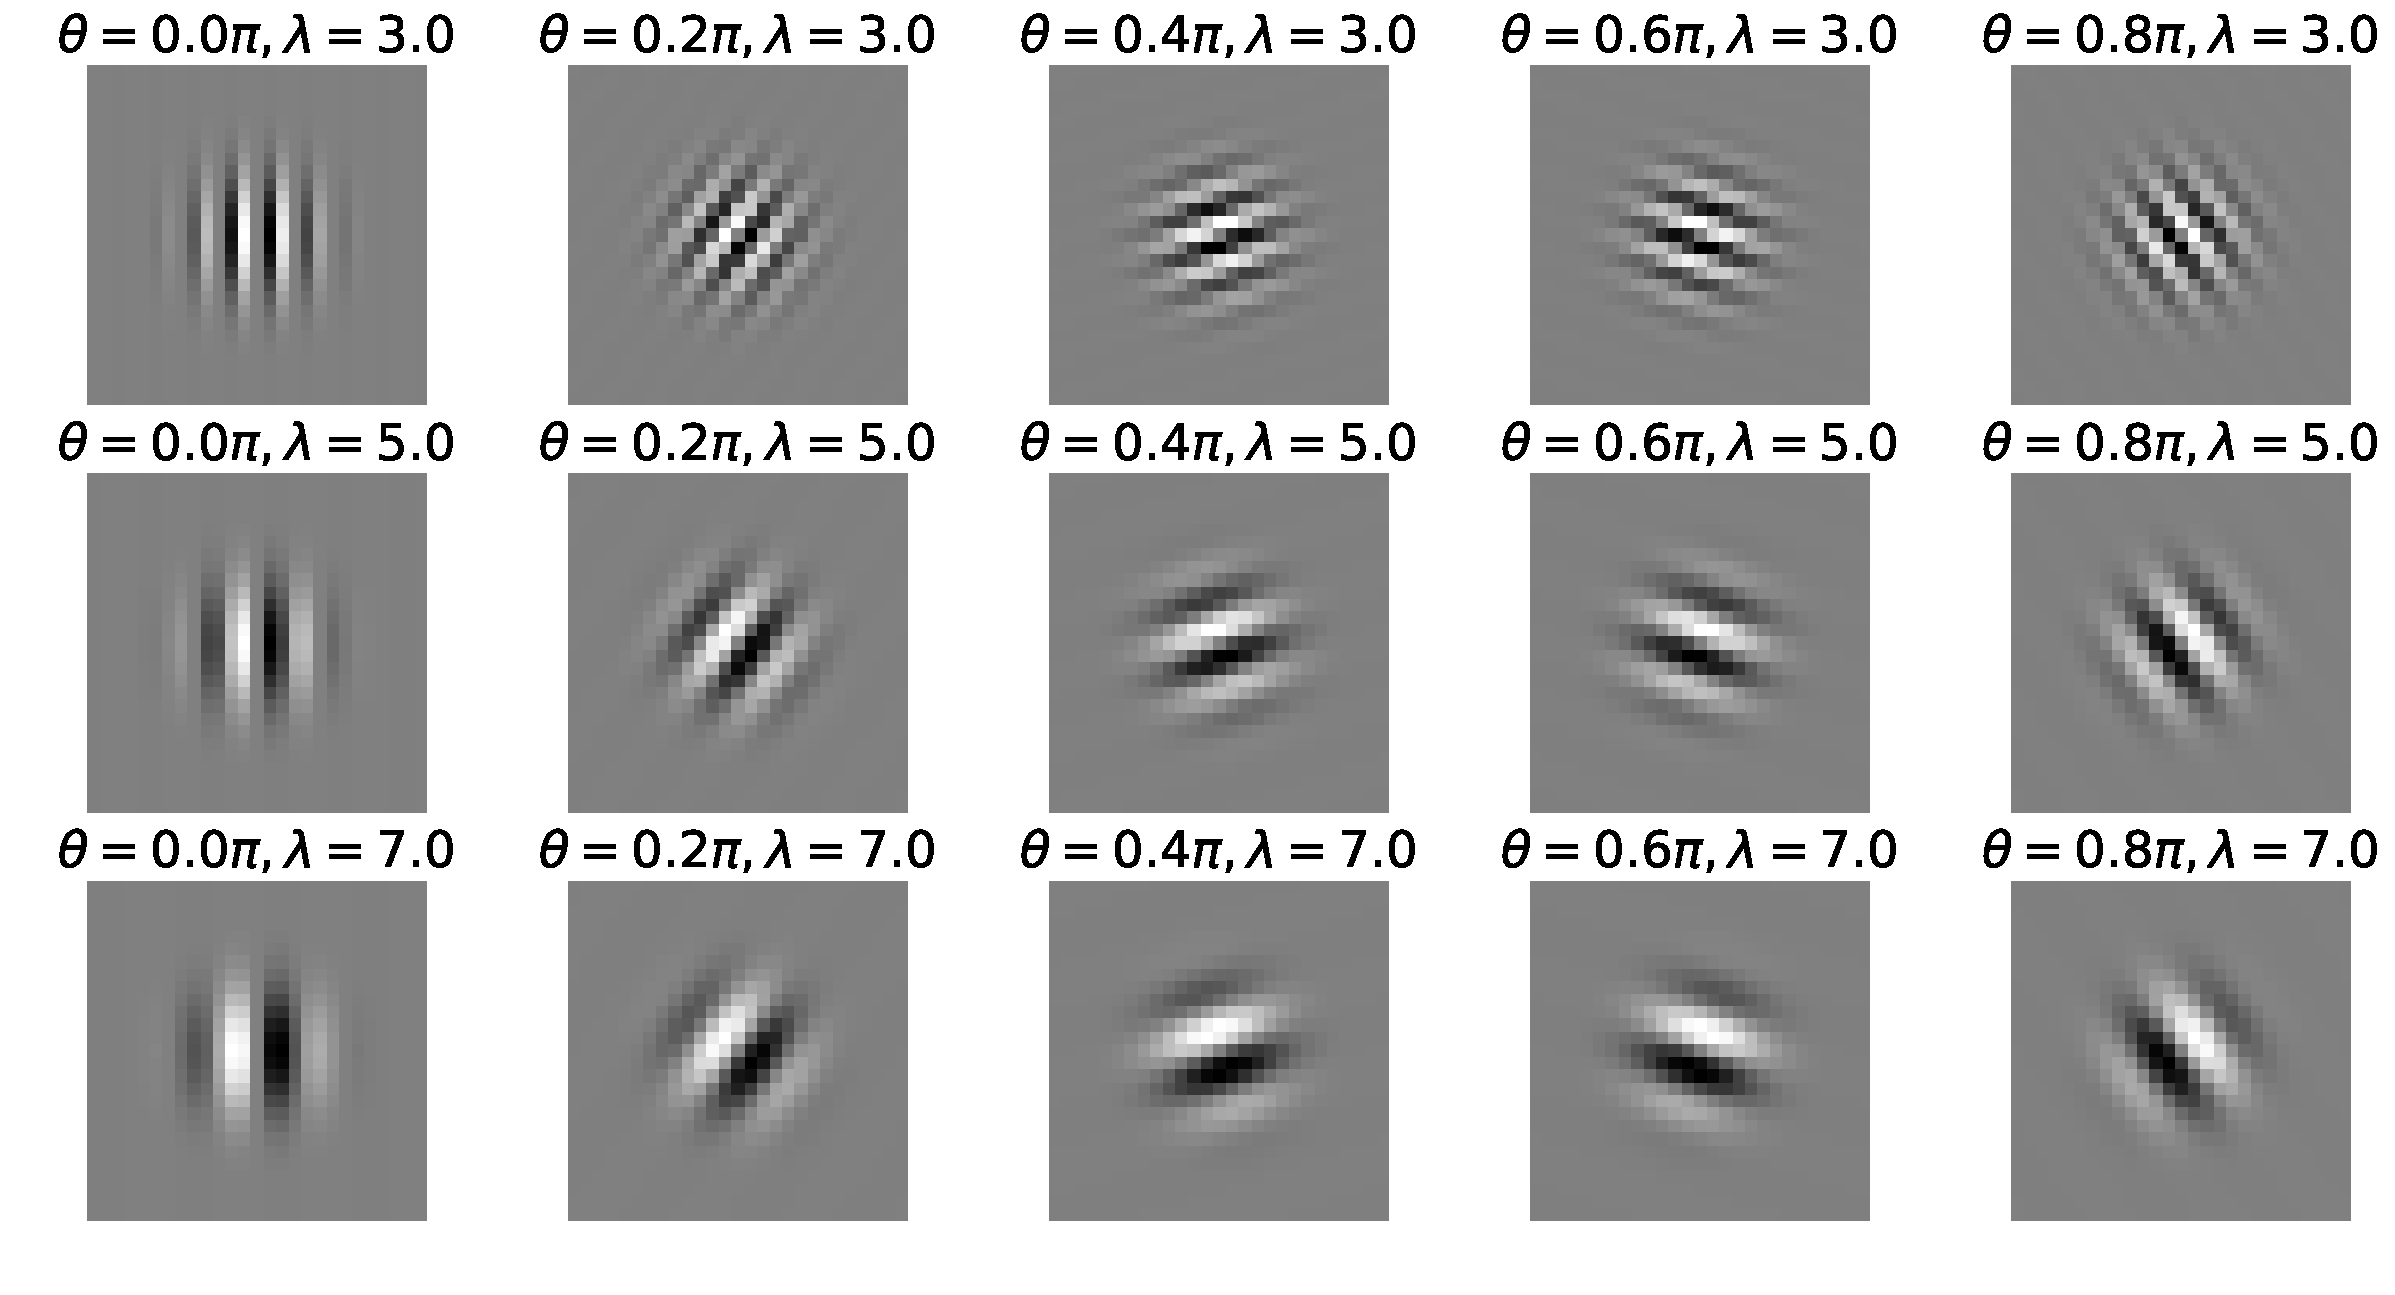
\includegraphics[width=.5\textwidth]{fig/gabor.pdf}
  \caption{\small Gabor wavelets constructed with $\psi=\pi/2,\sigma=3,\gamma=1$, variable angle $\theta$ and wavelength $\lambda$.}
  \label{fig:gabor}
\end{figure}

Gabor wavelets \cite{gabor} are widely used in image processing and feature extraction.
They are also present in the first layers of deep neural networks \cite{}, underlining their importance in early visual processing.

Gabor wavelets are parametrized as a composition of a Gaussian and Sinusoidal kernel.
A real valued gabor kernel is given as

\begin{align*}
    &g(x,y|\theta, \psi, \lambda, \sigma, \gamma) \\
    =& \exp\left(\frac{x'^2 + (\gamma y')^2}{-2\sigma^2}\right) \cos \left(\frac{2\pi}{\lambda}+\psi\right),
\end{align*}

with

\begin{align*}
  x' &= x \cos \theta + y \sin \theta \\
  y' &= -x \sin \theta + y \cos \theta.
\end{align*}

The parametrization includes the angle (filter rotation) $\theta$, phase offset $\psi$, wavelength $\lambda$, standard deviation $\sigma$ and skew $\gamma$.

Gabor filters with different settings for these parameters are depicted in figure~\ref{fig:gabor}.

\paragraph{Color opponent}

xxx

\paragraph{Color bias}

Humans seem to be attracted to a certain set of colors, which is why a color bias is implemented.

Color distance can be defined in different ways.

\subsubsection{Deep Neural Networks}

As deep learning becomes increasingly popular in image recognition \cite{LeCun2015}, it seems natural to adapt it to the task of saliency estimation.
In this report, I will focus on the work and models proposed by the Bethge lab \cite{Kummerer2017b,Kummerer2017a,Kummerer2014}, that are currently highest ranking on the MIT300 benchmark \cite{Bylinskii2015}.
Deep Gaze I \cite{Kummerer2014} and Deep Gaze II \cite{Kummerer2017b} make use of the feature maps computed by a deep neural network, in this case the VGG network \cite{Simonyan2014}.

In general, the overall approach of using a deep neural network is not fundamentally different from the previously discussed approaches.
Considering the framework presented above, a VGG model takes the role of $\F$, extracting feature maps based on the image, with a fixed set of parameters estimated by training on ImageNet data \cite{Simonyan2014}.

A readout network is then used to estimate a saliency map from the network outputs \cite{Kummerer2017b}, taking over the role of $W$ and $\phi$.

\subsubsection{Temporal Approaches}

\paragraph{Background Extraction}

For videos with a static background, a simple background extraction scheme can be used by computing the foreground components as the difference between each image and the temporal average.
Smoothing is applied to yield the final saliency map $S_B$:

\begin{equation}
  S_B^t = G_\sigma\left(x^t - \frac{1}{N} \sum_{\tau=1}^{N} x^\tau\right)
\end{equation}

\paragraph{Optical Flow}

Optical flow algorithms estimate a vector field ${\left(v_{i,j}\right)}_{i=1\dots W,j=1\dots H} \in \R^{W \times H \times 2}$ from a sequence of input images, where each $v_{i,j}$ denotes the direction in which the pixel $(i,j)$ is expected to move in the next timestep.
Optical flow can be computed using the approaches by Lucas and Kanade or more recently, using convolutional neural networks.
The computed optical flow map could be used as an input to the computation of the saliency maps.
In this work however, a simpler approach will be taken:
Given two images $x^t$ and $x^{t+1}$, an approximation to the temporal derivative will be used as a proxy for $\|v\|$:

\begin{equation}
    \|v\| \approx G_\sigma(x^{t+1}) - G_\sigma(x^{t}),
\end{equation}

where a gaussian smoothing function $G_\sigma$ was applied to alleviate high frequency noise between the images.

\subsection{Saliency Responses}

So far, we discussed different ways to extract feature maps of a given image.
In this section, an approach to combine feature extraction mechanisms into a saliency maps will be dicussed.

\subsection{Metrics}

As evaluation metrics, the commonly used mean-squared error (MSE) as well as the NSS score will be used, common for visual saliency \cite{Bylinskii2016,Bylinskii2015,Borji2015}.

\paragraph{Median squared error}

Given the human gaze fixation data median, $\mu' = (i, j)$ in
pixels coordinates, and the maximum salient response $\hat{\mu}$ from the model we
compute the total error of all frames $N$ as:

$$
\text{MSE}(\hat{\mu}, \mu') = \frac{1}{N} \sum_{i = 1}^N (\hat{\mu}_i - \mu'_i)^2
$$

\paragraph{NSS}

Given a binary map of fixation locations F (human data) and the saliency map S
(response from the model), the NSS measure is computed as:

$$
\text{NSS}(S,F) = \frac{1}{N} \sum_{i = 1}^N \overline{S}_i \odot F_i
$$

Where $N = \sum_i F_i$ is the total number of fixated pixels and $\overline{S} = \frac{S - \mu(S)}{\sigma(S)}$ is the normalized saliency map.
A value of 0 means means that it is chance (i.e., random), positive values shows correspondence and
negative values anti-correspondence.


\section{Experiments}

In this section, results for applying the previously introduced models are provided for both static images and video data.
For the exact parameters, please consider the provided reference implementation along with the supplementary material.

\subsection{Itty Koch Model}

Results for the Itty Koch Model applied to a collection of photographs as well as artificial stimuli is provided in figure~\ref{fig:ittykoch}.
The exact reaction to the artificial stimuli (rightmost images in the figure) is largely dependent on how the top-down modulation weights, i.e., the function $W$, is implemented.
For instance, for the fifth image depecting both highlighted and rotated instances of a ``5'', this directly influences whether the saliency response at the red five or the rotated 5 is more prominent.

\begin{figure*}[htp]
  \centering
  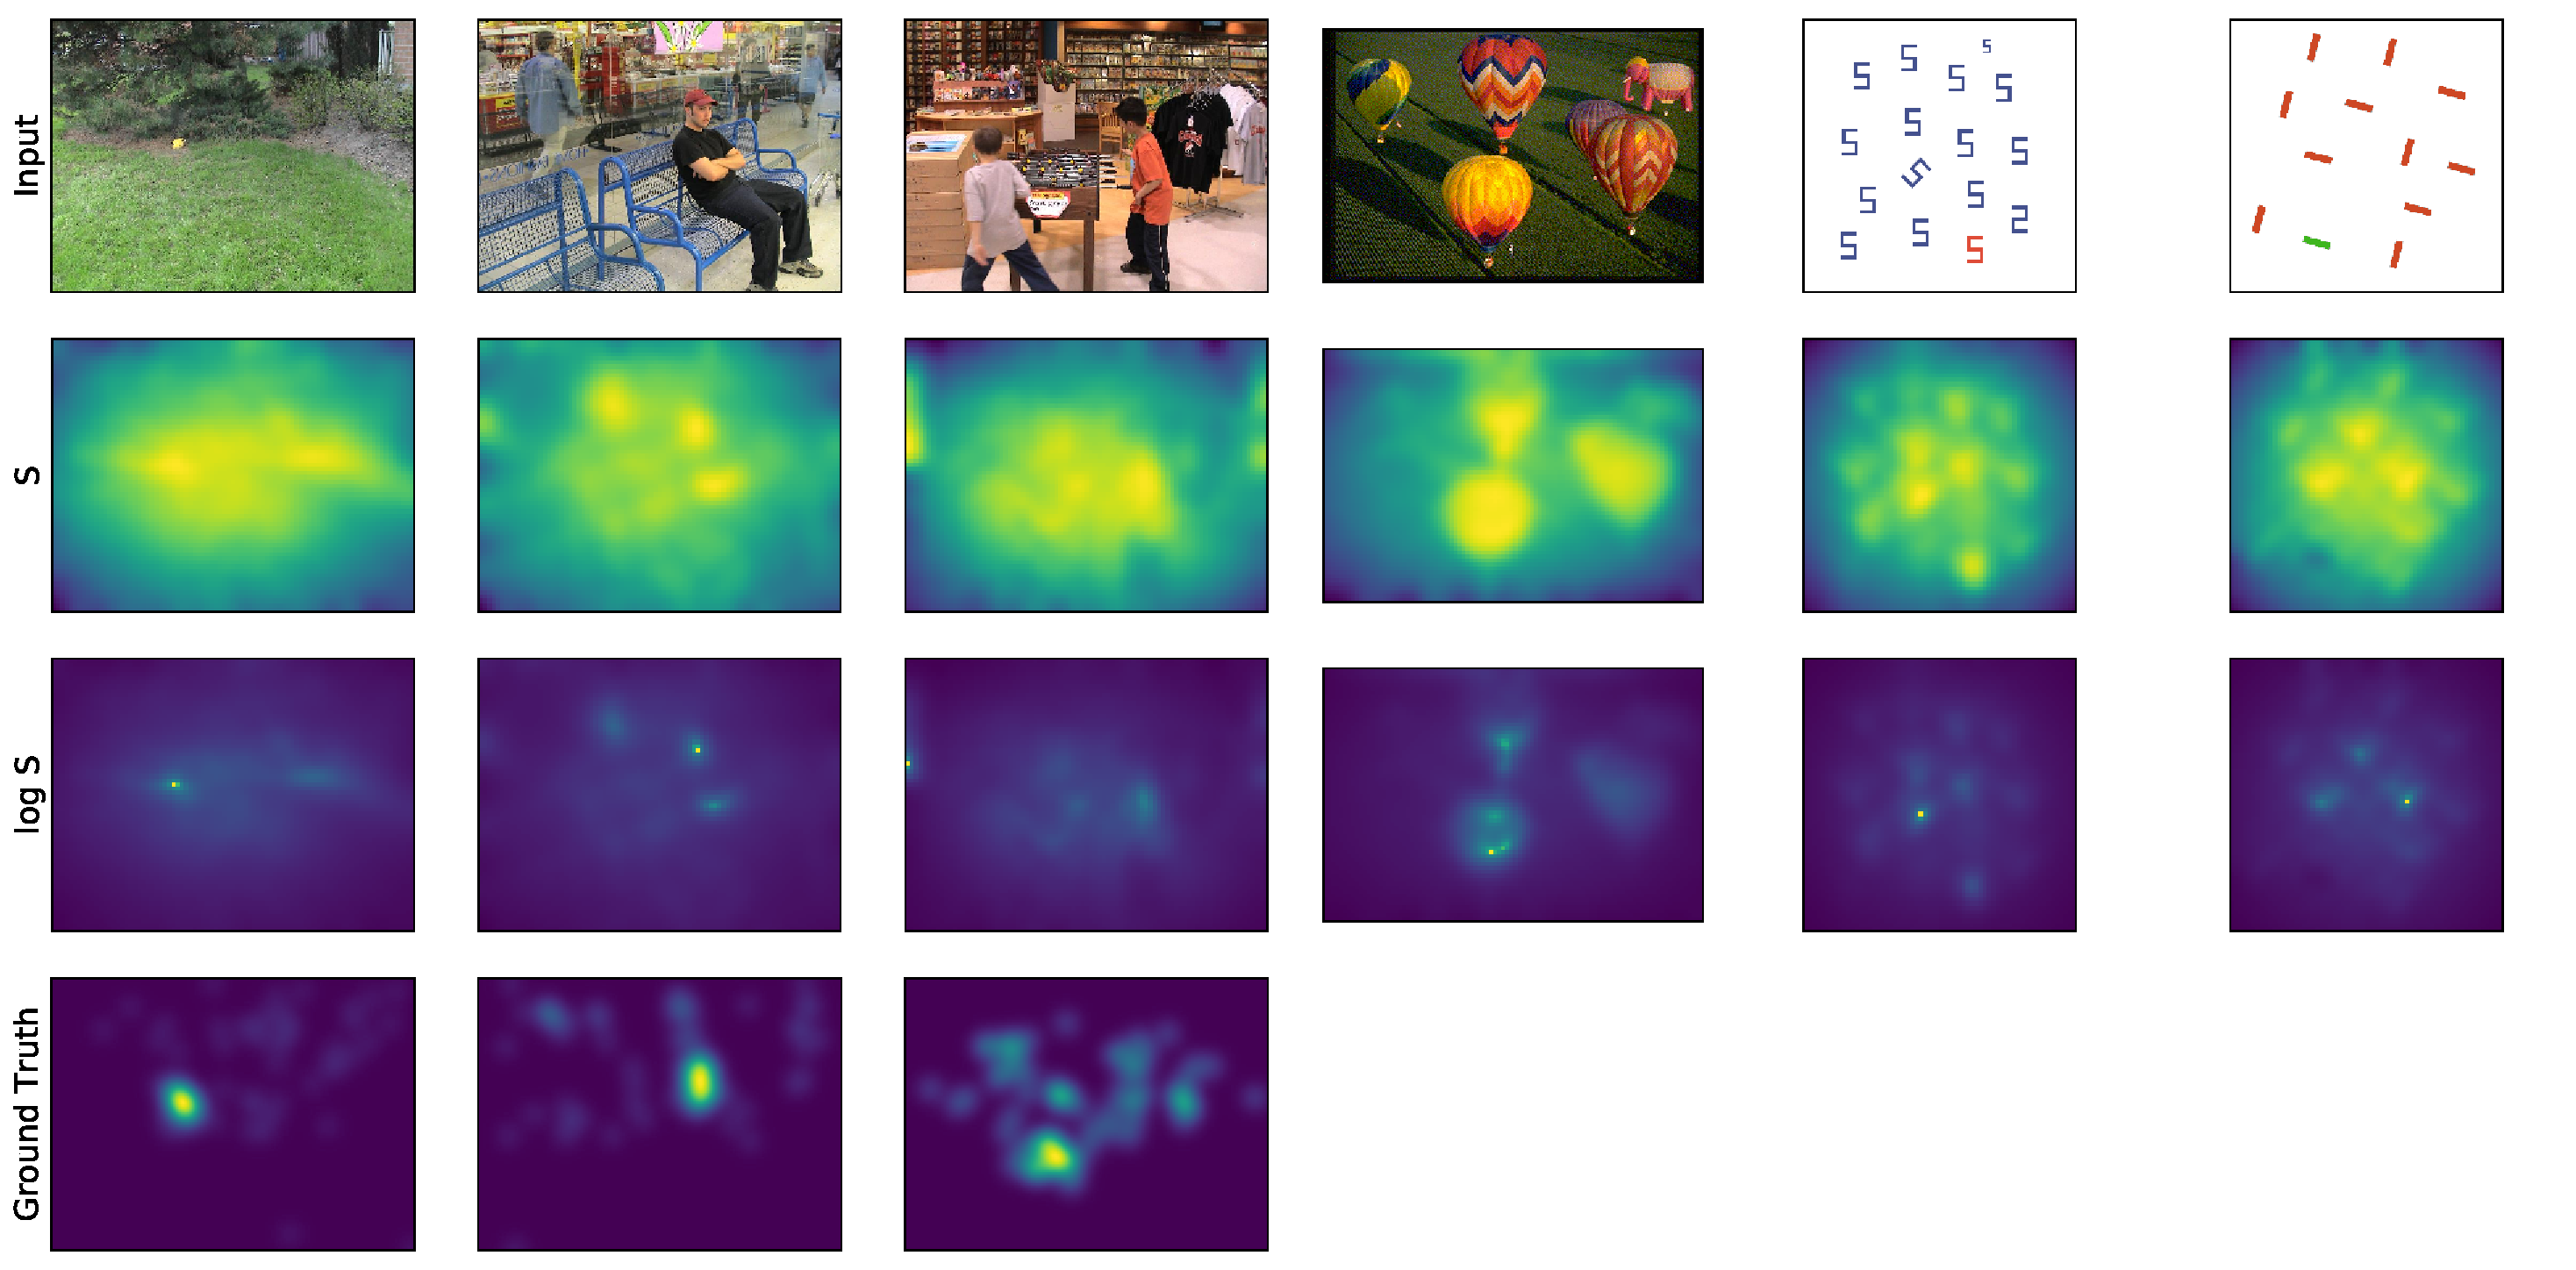
\includegraphics[width=\textwidth]{fig/output.pdf}
  \caption{\small
  Results for the Itty Koch \cite{Itty2000} model.
  As a simple strategy to get more focussed saliency map, we propose to compute the negative logarithm of the negative saliency output $S$, resulting in sharp peaks in the saliency map.
  With this representation, corrospondance to the ground truth becomes clear even when the saliency output is blurred substantially by the model.
  }
  \label{fig:ittykoch}
\end{figure*}

\subsection{Sequential Fixation with static images}

\begin{figure*}[tp]
  \centering
  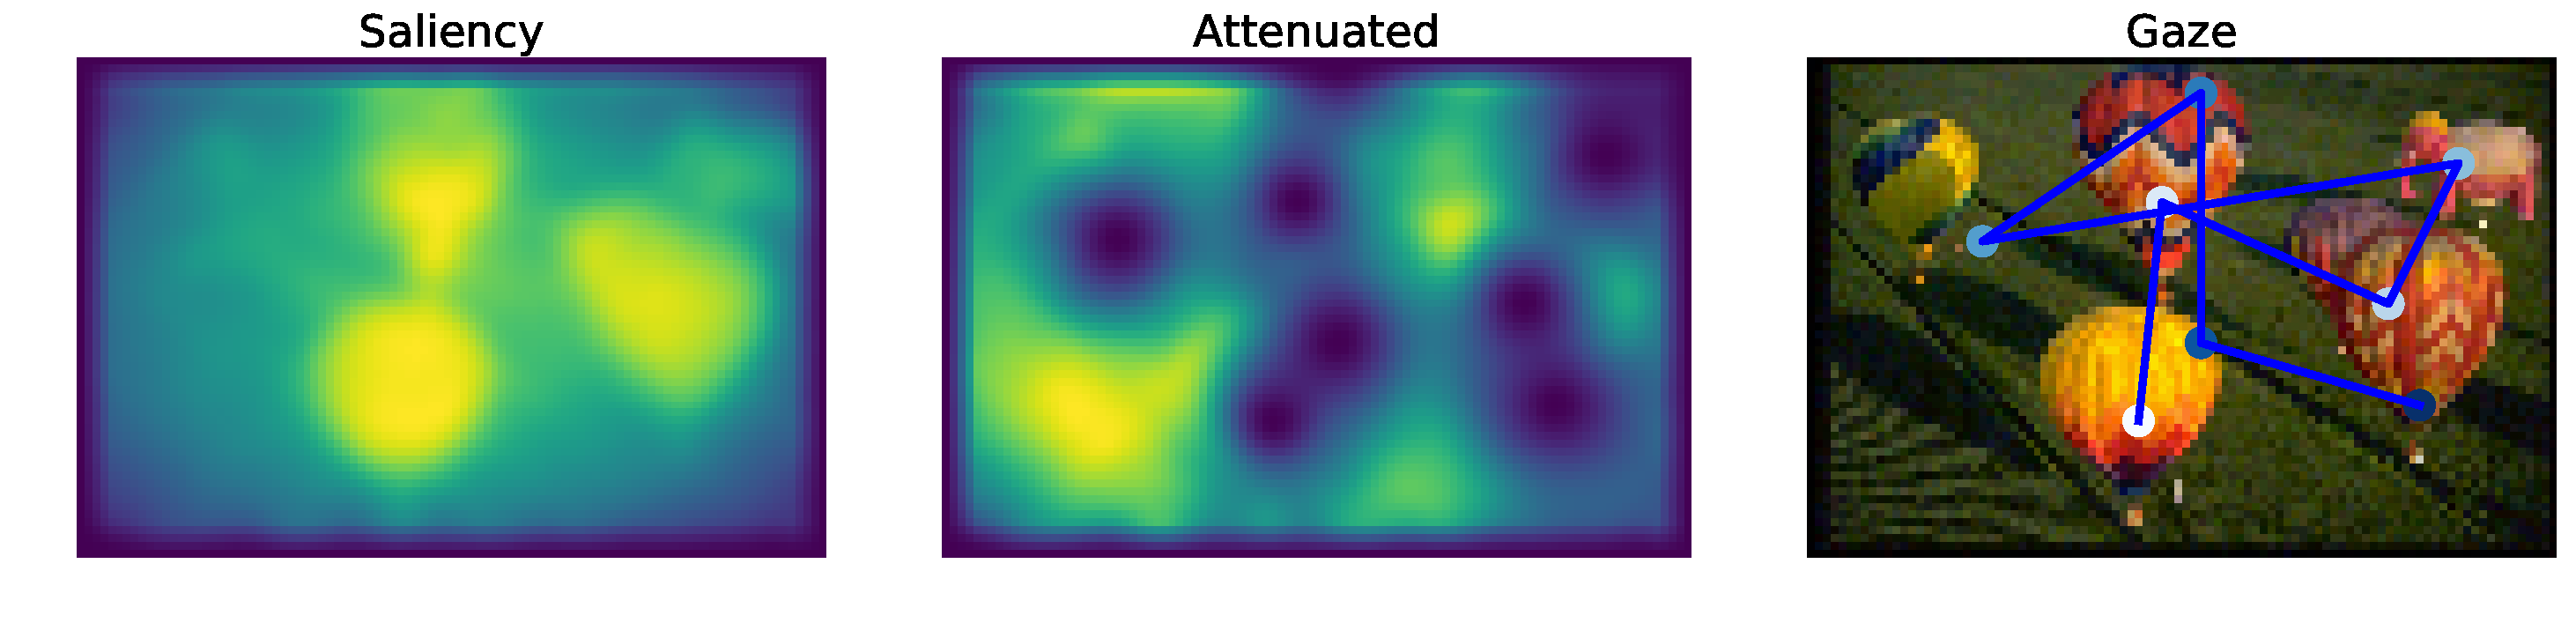
\includegraphics[width=\textwidth]{fig/sequence-3.pdf}
  \caption{\small
  Sequential fixation using sequential attention.
  Beginning from the saliency map, the point of maximum saliency is sampled.
  Afterwards, a region around this point is attenuated before the next point
  is sampled.
  A full list of prediction for different images can be found in the appendix figure~\ref{fig:app-sequential}.
  }
  \label{fig:sequential}
\end{figure*}

In this section, the implementation of a sequential attention mechanism is demonstrated.

A simple strategy which will be implemented here is using the maximally attended spot within the current saliency map $S^{(t)}$ to direct the gaze, i.e.,

\begin{equation}
f^{(t+1)} = \text{arg} \max_{i,j} S^{(t)},
\end{equation}

followed by
\begin{equation}
S^{(t+1)} = (1 - G_\sigma(\delta_{i,j})) \odot S^{(t)},
\end{equation}

where $\delta_{i,j}$ is an image with pixel $(i,j)$ being the only non-zero pixel set to 1.
Results for sequential fixation are depicted in Figure~\ref{fig:sequential} and for more images in the appendix, Figure~\ref{fig:app-sequential}.

\subsection{Sequential Trajectory of gaze fixation on a video}

The DeepGazeII and ICF models from \cite{Kummerer2017b} were used on all videos for an upper baseline \footnote{For this work, the tensorflow implementation provided at \texttt{deepgaze.bethgelab.org} was integrated into the experimental framework}.
For a lower baseline, two models using temporal differences or background extraction were used.
For the human baseline, an 18-fold cross validation was run by using the trajectory of one subject as the ``prediction'' of a model and tested against the remaining 17 subject's gaze trajectories.
Mean and standard deviation of this human baseline is also reported.

A graphical comparison is given in Figure~\ref{fig:todo}, the exact values are given in Table~\ref{tbl:todo}.

\section{Discussion}

The classic, but slightly simplified Itty Koch model only relying on hand-crafted features could already explain a range of test stimuli, such as color bias and selection of high frequency information in the image using gabor wavelets.

Replacing the hand-crafted feature extraction mechanisms with features learned for object classiciation, further improvement is possible.
On temporal data, using the difference between saliency responses of different models to detect changes in saliency was used in this report.

Improvements are likely if the used models are explicetly designed to take into account temporal information (e.g., by the use of temporal filters or optical flow estimation).

\section{Supplementary Material}

The implementation of the models along with supplementary figures is available at \texttt{github.com/stes/saliency}.
Implementation was performed in Python, using Tensorflow for running the Deep Gaze II and ICF \cite{Kummerer2017b} models.
The Itty Koch model was not fully implemented according to the original work \cite{Itti2000}, however the overall model structure is consistent.

\bibliographystyle{plain}
\bibliography{refs}

\clearpage
\begin{appendix}
\onecolumn

\section{Sequential Fixation}
  \begin{figure}[ht]
    \centering
    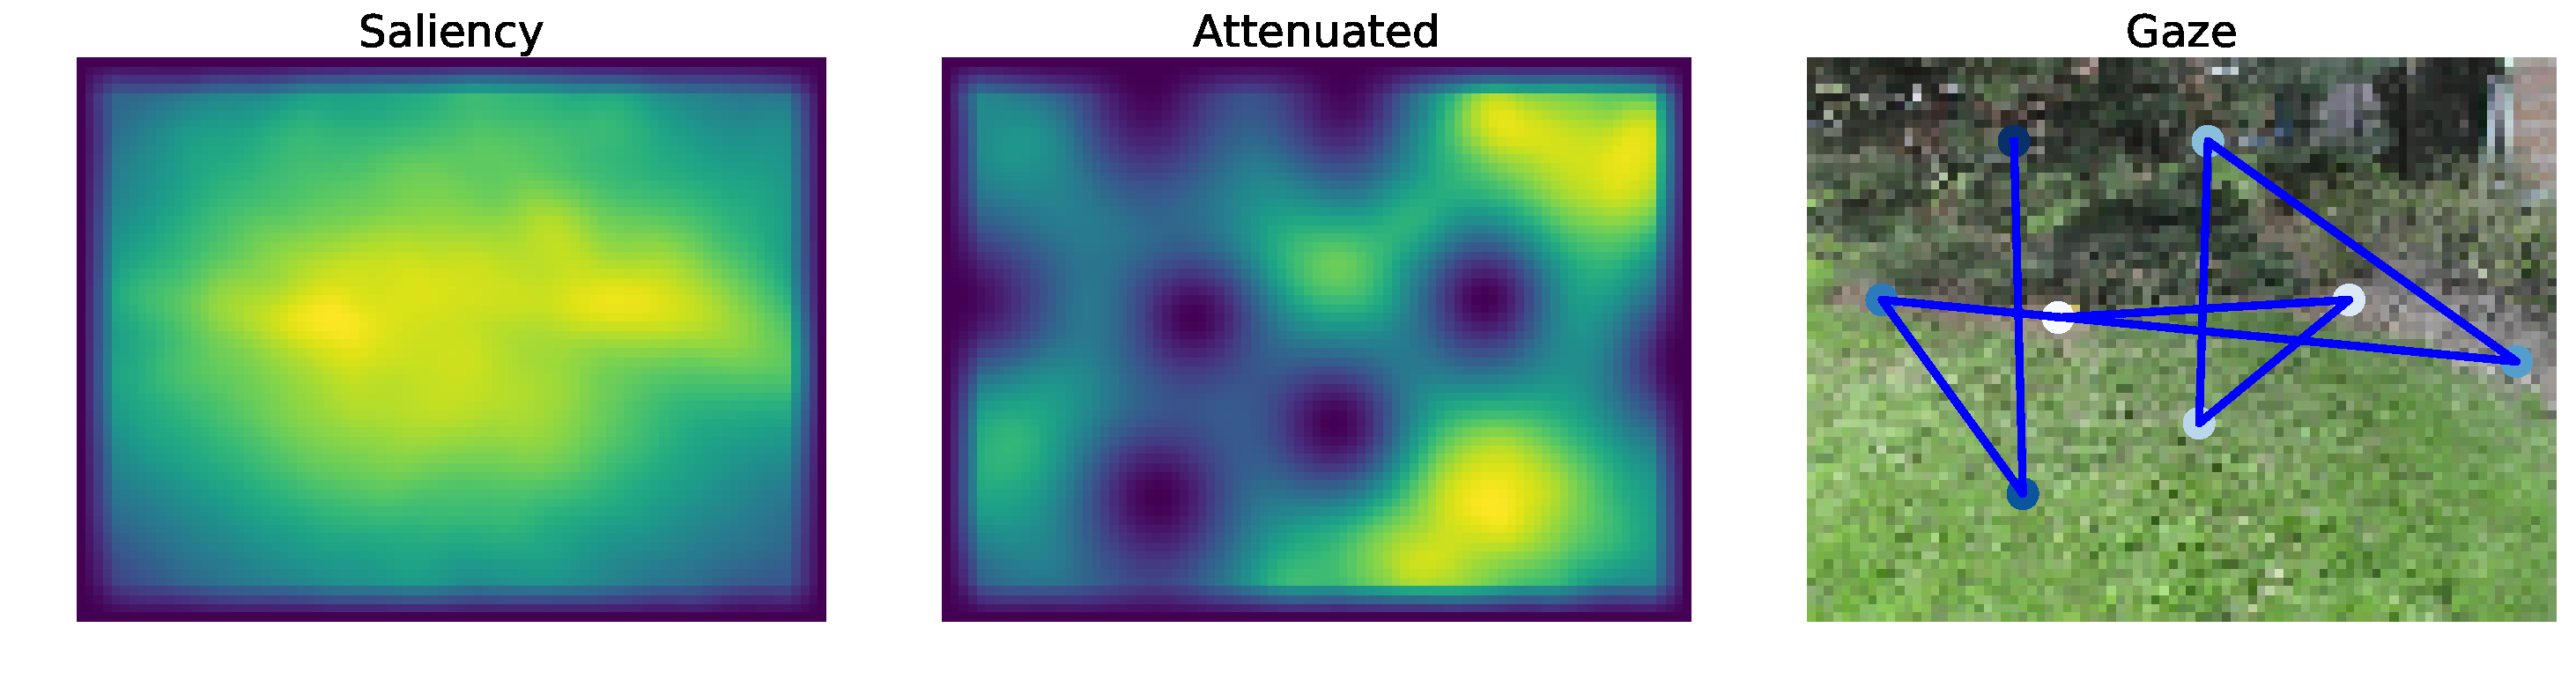
\includegraphics[width=.8\textwidth]{fig/sequence-0.pdf}
    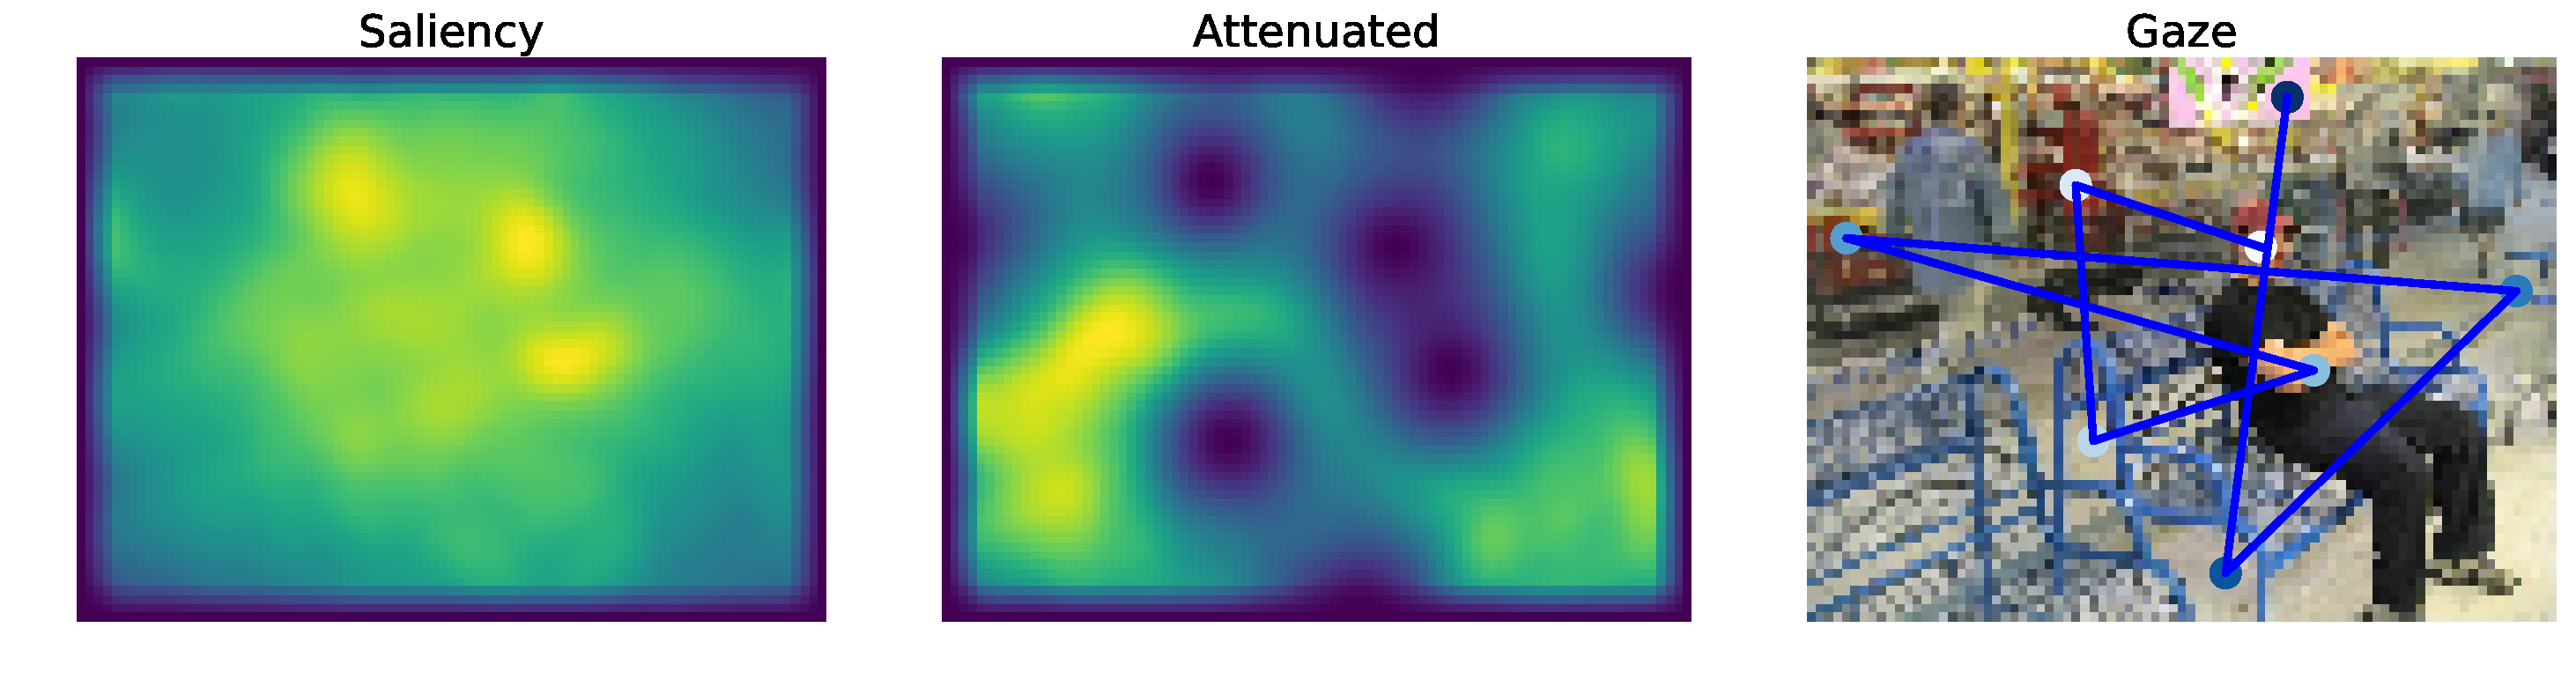
\includegraphics[width=.8\textwidth]{fig/sequence-1.pdf}
    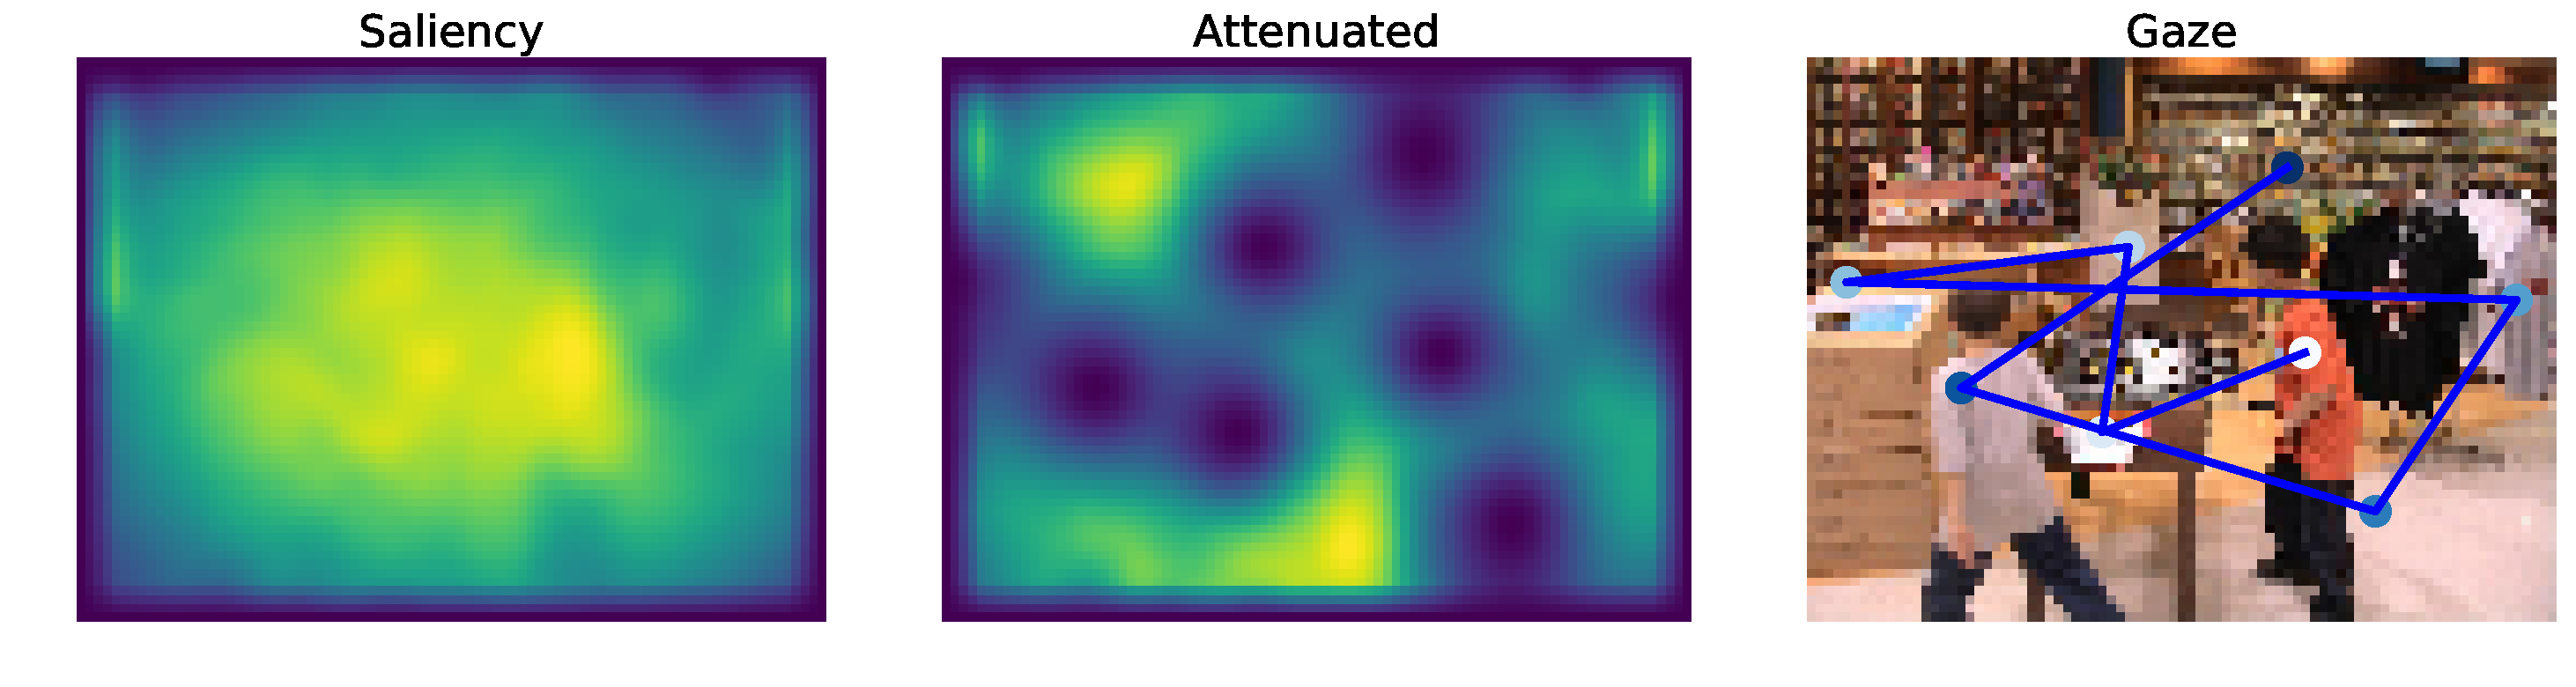
\includegraphics[width=.8\textwidth]{fig/sequence-2.pdf}
    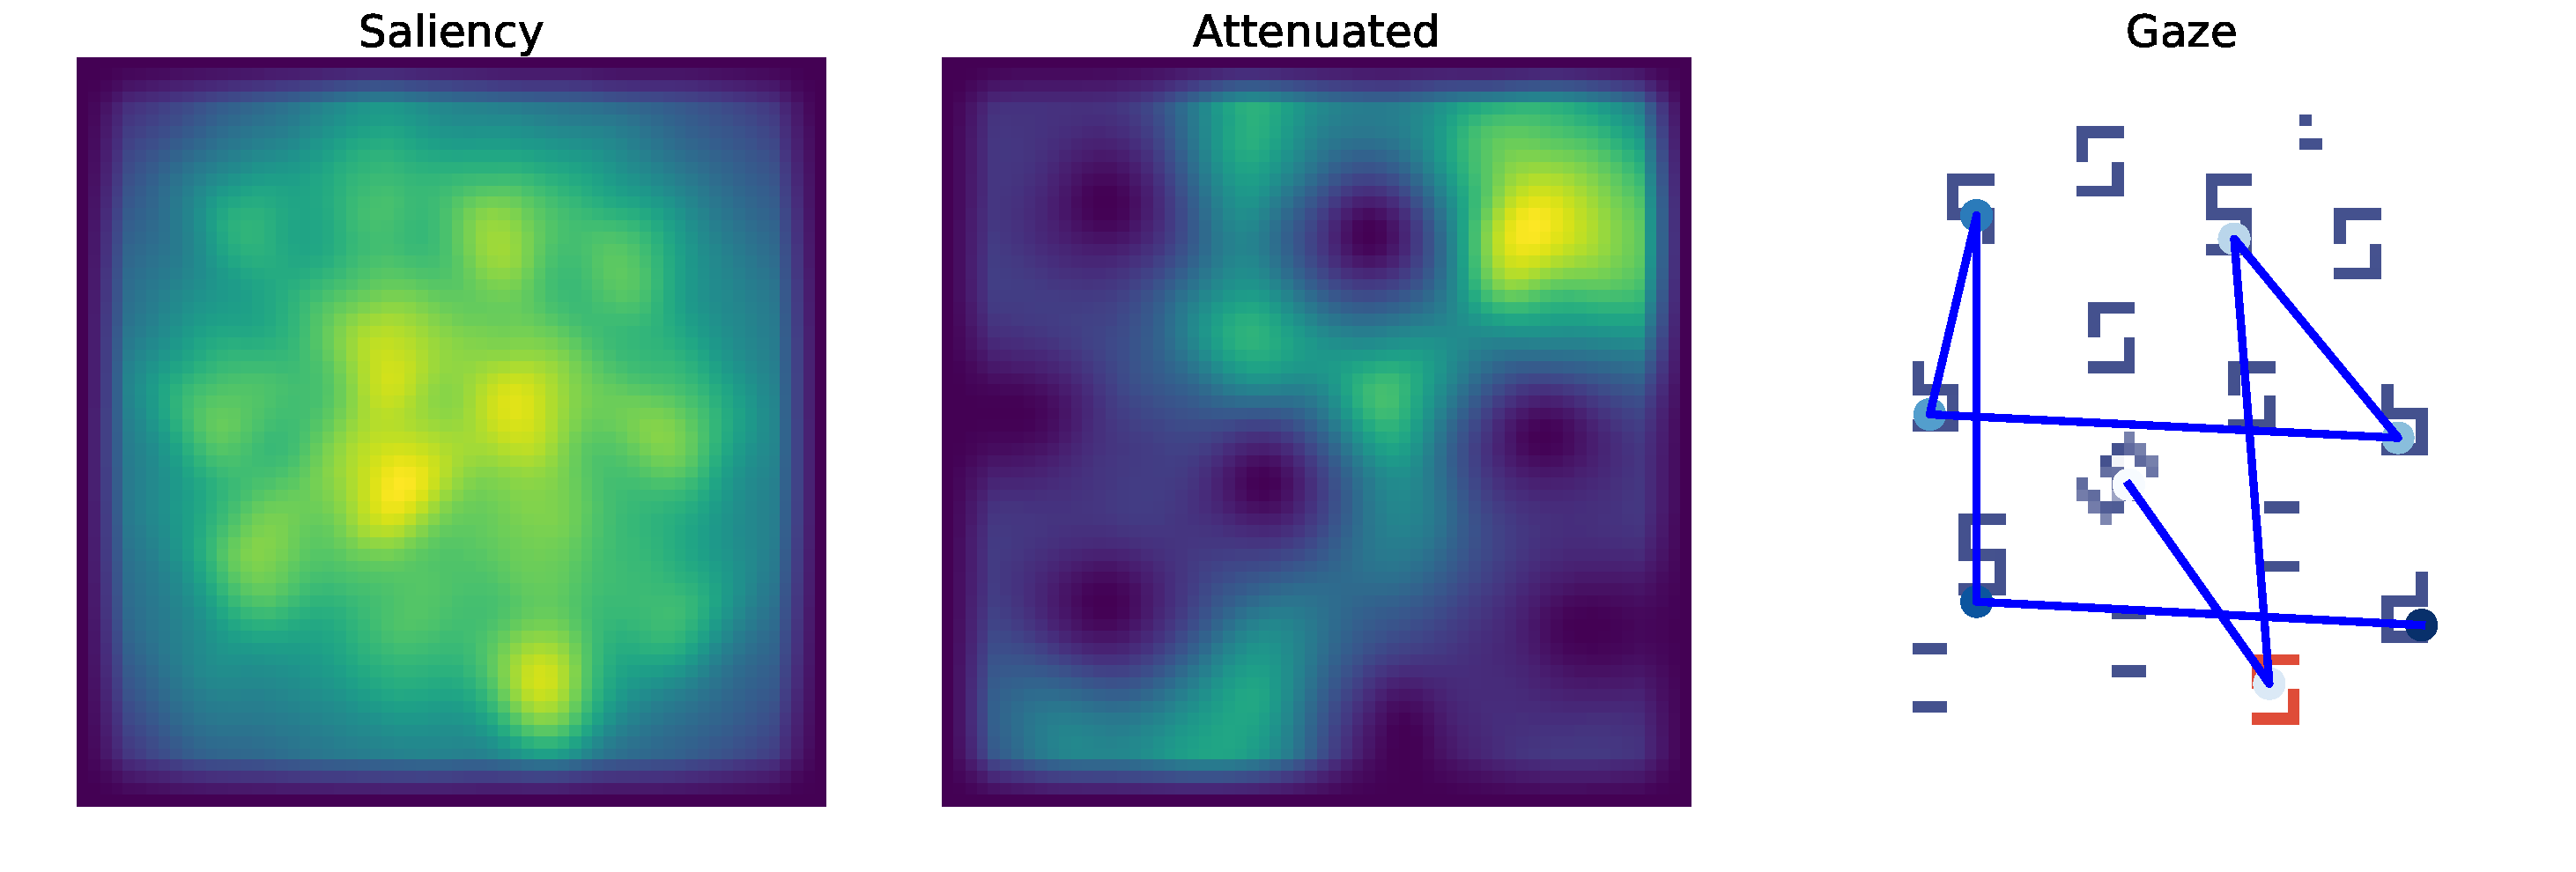
\includegraphics[width=.8\textwidth]{fig/sequence-4.pdf}
    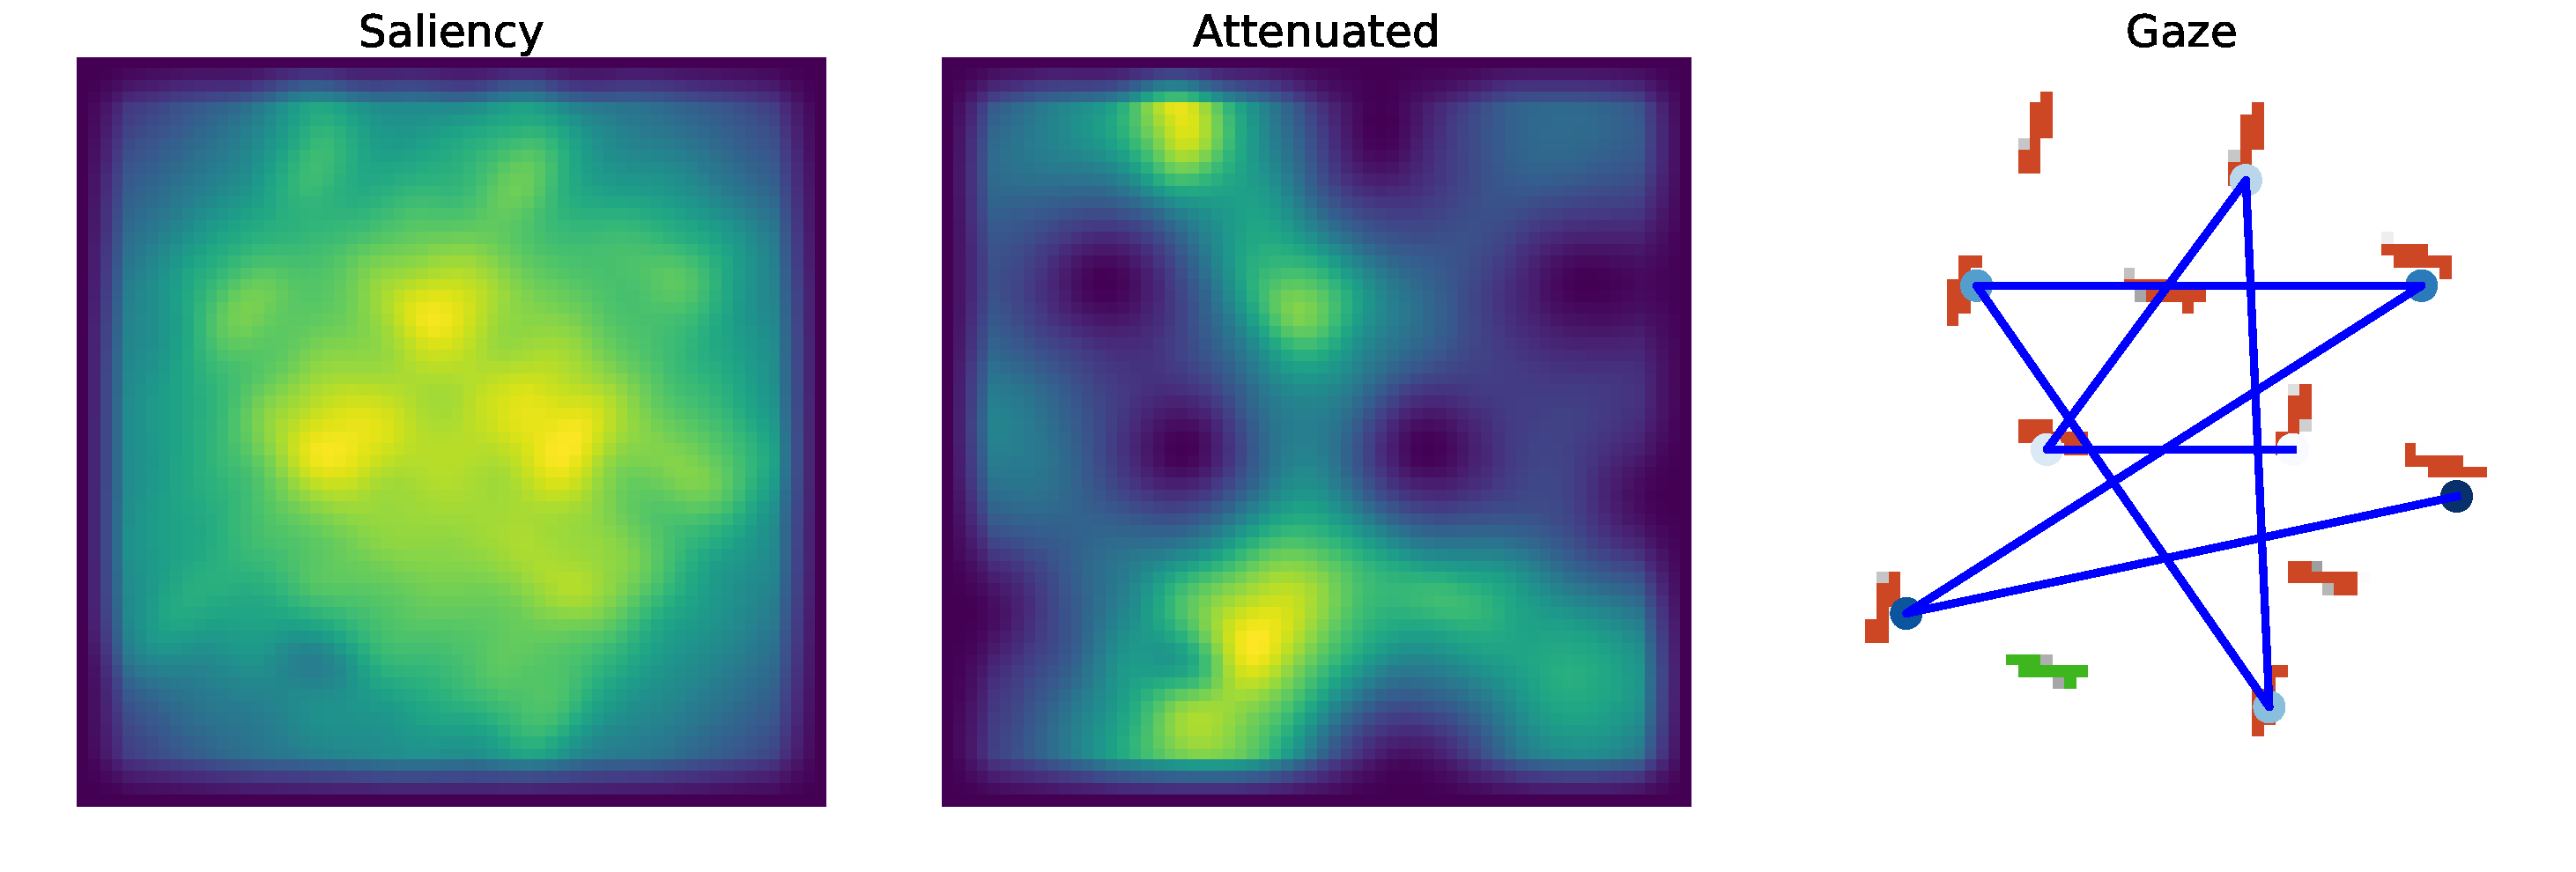
\includegraphics[width=.8\textwidth]{fig/sequence-5.pdf}
    \caption{Sequential fixation for all images, including test stimuli.
    The fixation sequence is color-coded from first fixation (White) to last fixation (Blue).
    }
    \label{fig:app-sequential}
  \end{figure}

\clearpage

\end{appendix}

\end{document}
